\chapterimage{Pictures/Ausberto/3_analise.png} % Table of contents heading image

\begin{comment}
        Prof. Dr. Ausberto S. Castro Vera
        UENF - CCT - LCMAT - Curso de Ciência da Computação
        Campos, RJ,  2022
        Disciplina: Análise e Projeto de Sistemas
        Aluno: João Vítor Fernandes Dias
    \end{comment}

\chapter{Etapa de Análise}
    Neste capítulo descrevemos algumas etapas da análise do projeto de sistema acadêmico.
    
    \begin{comment}
    
    
    \section{Requisitos do Sistema} % 4) Lista de Requisitos: 80 + 32 + 8
        Nesta seção apresenta-se a lista de requisitos exigidos pelo sistema.
        
        \subsection{Requisitos} % 80
            \begin{enumerate}
                \item Acesso online da plataforma web % \item [MOBILIDADE]
                \item Acesso pelo app
                \item Acesso por computador
                \item Acesso por smartphone
                \item Analista de requisitos
                \item Analista de sistemas
                \item Análise semestral da situação dos softwares e equipamentos
                \item Ar condicionado
                \item Arquiteto de Software
                \item Auxiliar de manutenção
                \item Avaliador de qualidade % \item [PESSOAS]
                \item Backup dos dados
                \item Banco de dados das matérias ofertadas
                \item Cabos de energia % \item [HARDWARE]
                \item Cabos Ethernet
                \item Cadastro de alunos
                \item Cadastro de disciplinas
                \item Cadastro de informações do sistema através de documentos de requisição % \item [PROCEDIMENTOS E METODOLOGIA]
                \item Cadastro de professores
                \item Cadastro de Turmas
                \item Cargos exercidos por cada professor
                \item Contratação de domínio
                \item Cálculo semestral de demanda por matérias
                \item Código único para cada usuário
                \item Desenvolvimento com metodologia SCRUM % \item [PROCEDIMENTOS E METODOLOGIA]
                \item Designer
                \item Disponibilidade de horários dos alunos
                \item Disponibilidade de horários dos professores
                \item Endereço dos alunos
                \item Engenheiro de Software
                \item Enviar e-mail para alunos
                \item Estabilizadores
                \item Exclusão de matérias
                \item Faxinas semanais nos servidores e salas
                \item Filtros de linha
                \item Gerar extratos
                \item Gerente de projeto % \item [PESSOAS]
                \item Gestores com capacidade de alteração total do sistema % \item [SOFTWARE]
                \item Histórico de notas
                \item Histórico de todas as notas
                \item Histórico de todas as turmas
                \item Impressora multifuncional
                \item Impressora multifuncional % \item [NUVEM]
                \item Licença antivírus
                \item Licença SO proprietário
                \item Listagem de todas as salas por centro
                \item Listagem de todos os centros
                \item Login e senha para cada um dos usuários
                \item Manutenção dos equipamentos
                \item Matrículas dos alunos
                \item Matérias que cada professor pode ministrar
                \item Microcomputadores com acesso a internet para funcionários do sistema % \item [HARDWARE]
                \item Mobília geral
                \item Monitores
                \item Mouses
                \item No-breaks
                \item Nome dos alunos % \item [BANCO DE DADOS]
                \item Notas obtidas
                \item Pacotes LibreOffice
                \item Passar atividades para alunos % \item [SOFTWARE]
                \item Período de abertura dos centros % \item [BANCO DE DADOS]
                \item Portabilidade de dados % \item [MOBILIDADE]
                \item Prioridade nos processos presenciais
                \item Programadores
                \item Projetista
                \item Provas feitas
                \item Requisição de alteração de nota
                \item Requisição de cadastro de turma
                \item Requisição de cadastro no sistema % \item [DOCUMENTAÇÃO]
                \item Roteador Wireless
                \item Secretária
                \item Seleção automática da grade de horários
                \item Seleção de turma disponível
                \item Seleção manual da grade de horários
                \item Servidor reserva % \item [NUVEM]
                \item Servidores próprios
                \item Site e App com modo escuro seletivo
                \item Smart TV
                \item Solicitação de alteração de curso % \item [DOCUMENTAÇÃO]
                \item Solicitação de trancamento
                \item Switch
                \item Teclados
                \item Turmas
                \item Técnico de redes
            \end{enumerate}
        \subsection{Definição de Requisitos} % 32
            \begin{enumerate}
                \item Acesso online da plataforma web - O sistema deve ser acessível pelo APP % \item [MOBILIDADE]
                \item Acesso pelo app - O sistema precisa ser acessível pelo APP
                \item Acesso por computador - É necessário que o sistema possa ser acessado pelo computador
                \item Acesso por smartphone - É necessário que o sistema possa ser acessado pelo smartphone
                \item Análise semestral da situação dos softwares e equipamentos - A análise do software permite buscar e corrigir falhas na segurança
                \item Backup dos dados - Caso o servidor original filho caia, ainda há um backup
                \item Cadastro de informações do sistema através de documentos de requisição - Possível de se fazer requisições físicas para alterações nas informações do sistema digital % \item [PROCEDIMENTOS E METODOLOGIA]
                \item Cargos exercidos por cada professor - Professores podem acumular mais cargos do que deveria poder. Essa foi uma forma de tornar mais transparente essa informação
                \item Cálculo semestral de demanda por matérias - O sistema irá analisar automaticamente qual a demanda de matéria para todos os alunos
                \item Designer - O Designer irá cuidar da parte gráfica e apresentação da plataforma
                \item Faxinas semanais nos servidores e salas - Para que os equipamentos comprados sejam longevos, é necessário haver faxinas semanais
                \item Gestores com capacidade de alteração total do sistema - É necessário que alguns dos gestores tenham permissão máxima no sistema % \item [SOFTWARE]
                \item Histórico de notas - Documento físico e  histórico de notas de cada aluno
                \item Impressora multifuncional - Impressora conectada à rede interna para poder imprimir os documentos que forem necessários % \item [HARDWARE]
                \item Listagem de todas as matérias - A listagem de todas as matérias se encontra na base de dados do sistema
                \item Login e senha para cada um dos usuários - Cada usuário terá sua própria senha e login para acessar seus dados
                \item Matrículas dos alunos - Deve haver apenas uma matricula por aluno % \item [BANCO DE DADOS]
                \item Microcomputadores com acesso a internet para funcionários do sistema - Para que os desenvolvedores e os funcionários mexam no sistema, é ideal que sejam disponibilizados microcomputadores para o serviço
                \item Notas obtidas - É essencial saber a nota para que o sistema possa calcular a demanda corretamente
                \item Portabilidade de dados - Permite que todas as informações do usuário sejam exportadas para um arquivo JSON ou PDF que tem todas as informações que queira portar 
                \item Prioridade nos processos presenciais - No caso da pessoa que lida com as requisições, ela deve focar em resolver aquelas que forem feitas presencialmente o quanto antes.
                \item Programadores - Programadores programarão o sistema % \item [PESSOAS]
                \item Requisição de cadastro de turma - Documento físico para que o aluno entre em alguma turma
                \item Requisição de cadastro no sistema - Documento físico para se cadastrar no sistema % \item [DOCUMENTAÇÃO]
                \item Roteador Wireless - Dispositivo utilizado para disponibilizar internet sem fio em área
                \item Secretária - A secretária irá atende às solicitações de ajuda e de requisições
                \item Seleção automática da grade de horários - O sistema irá analisar automaticamente a grade mais otimizada para todos os alunos
                \item Servidor reserva - O servidor reserva na nuvem serve como um outro sistema, que pode ser ativado caso o principal dê problema % \item [NUVEM]
                \item Servidores próprios - Servidores físicos próprios localizados na instituição para servir como base dos sites e aplicativos
                \item Solicitação de alteração de curso - Documento físico necessário para mudar de curso
                \item Solicitação de trancamento - Documento físico necessário para trancar a matrícula
                \item Turmas - O banco de dados armazena todas as turma que cursaram as disciplinas
                \item Técnico de redes - Irá cuidar da conexão dos fios e equipamentos e auxiliar o banco de dados a tar estabilidade de alguma forma
            \end{enumerate}
        \subsection{Especificação de Requisitos} % 8
            \begin{enumerate}
                \item Impressora multifuncional
                    \begin{enumerate}
                        \item Acessar a impressora pela rede externa
                        \item Acessar a impressora pela rede interna
                        \item Conectar a impressora a rede
                        \item Configurar a impressora
                    \end{enumerate}
                \item Gestores com capacidade de alteração total do sistema % \item [S
                    \begin{enumerate}
                        \item Acessar a sua conta do sistema acadêmica
                        \item Colocar a senha especial
                        \item Programadores gerarão senhas para que gestores possam fazer uso irrestrito de poder
                    \end{enumerate}
                \item Seleção manual da grade de horários
                    \begin{enumerate}
                        \item Ir até a área de gerência de turmas
                        \item Logar com seu usuário e senha de gestor
                        \item Mover a grade de quem quiser. Assim analisando em tempo real quais mudanças seriam ruins
                    \end{enumerate}
                \item Seleção automática da grade de horários
                    \begin{enumerate}
                        \item Clicar em buscar soluções ótimas
                        \item Ir até a área de gerência de turmas
                        \item Logar com seu usuário e senha de gestor
                    \end{enumerate}
                \item Gerar extratos
                    \begin{enumerate}
                        \item Clicar em gerar extratos, o extrato surge na impressora.
                        \item Ir até a área de gerência de turmas
                        \item Logar com seu usuário e senha de gestor
                        \item Selecionar um dos alunos
                        \item Selecionar uma das turmas
                    \end{enumerate}
                \item Backup dos dados
                    \begin{enumerate}
                        \item Baixar os dados gerados
                        \item Enviar todas as cópias dos dados gerados para a nuvem
                        \item Preparar o retorno dos dados
                    \end{enumerate}
                \item Histórico de notas
                    \begin{enumerate}
                        \item Lista de matérias concluídas e suas respectivas notas
                        \item pode ser impresso como substituto do "gerar extrato"
                    \end{enumerate}
                \item Portabilidade de dados % \item [MOBILIDADE]
                    \begin{enumerate}
                        \item Organizar cada parcela de dados em sua forma primitiva
                        \item Unificar os dados como um arquivo de texto JSON
                    \end{enumerate}
            \end{enumerate}
    
    \section{Stakeholders e Pontos de Vista} % 5 de abr. 12:00
        Abaixo serão descritos os stakeholders e pontos de vista.
    
        \subsection{Stakeholders}
            \begin{enumerate}
                \item Alunos
                \item Analista de requisitos
                \item Analista de sistemas
                \item Arquiteto de Software
                \item Auxiliar de manutenção
                \item Avaliador de qualidade
                \item Designer
                \item Engenheiro de Software
                \item Gerente de projeto
                \item Professores
                \item Programadores
                \item Projetista
                \item Secretária
                \item Técnico de redes
            \end{enumerate}

        \subsection{Pontos de Vista}
            \subsubsection{Diretos}
                \begin{itemize}
                    \item Alunos
                        \begin{itemize}
                            \item Inscrição em matérias
                            \item Pesquisar ementas
                            \item Remover matérias
                            \item Solicitação de requerimentos
                            \item Ver extrato
                        \end{itemize}
                    \item Professores
                        \begin{itemize}
                            \item Colocar as notas
                            \item Criar turmas
                            \item Disponibilizar conteúdo
                            \item Finalizar a turma
                            \item Ver lista de alunos da turma
                        \end{itemize}
                    \item Programadores
                        \begin{itemize}
                            \item Acesso ao banco de dados
                            \item Acesso ao código
                            \item Adicionar alunos
                            \item Adicionar professores
                            \item Alterar cargos
                        \end{itemize}
                    \item Gerentes de projeto
                        \begin{itemize}
                            \item Busca de problemas
                            \item Busca de requisitos
                            \item Definição das próximas tarefas
                            \item Organização dos funcionários
                            \item Resolução de problemas
                        \end{itemize}
                    \item Coordenadores
                        \begin{itemize}
                            \item Criar turmas
                            \item Deletar turmas
                            \item Modificar alunos
                            \item Modificar horários
                            \item Modificar professores
                        \end{itemize}
                \end{itemize}
            \subsubsection{Indiretos}
                \begin{itemize}
                    \item Centros Acadêmicos    % 15/05/2022 - 21h24
                        \begin{itemize}
                            \item Acesso a quantidade de alunos do curso do Centro Acadêmico 
                            \item Acesso a listagem de alunos do curso do Centro Acadêmico
                            \item Agenda de eventos estipulados para o curso do Centro Acadêmico
                            \item Marcação de eventos
                            \item Listagem de matérias de professores
                        \end{itemize}
                    \item Gestão financeira
                        \begin{itemize}
                            \item Listagem de bolsistas de Assistência Administrativa
                            \item Listagem de bolsistas de Extensão
                            \item Listagem de bolsistas de Iniciação Científica
                            \item Quantidade de alunos de cada Centro
                            \item Valor das bolsas a serem pagas
                        \end{itemize}
                    \item Prefeitura da Universidade
                        \begin{itemize}
                            \item Agenda de eventos estipulados para todos os cursos
                            \item Listagem de professores
                            \item Quantidade de alunos de cada Centro
                            \item Quantidade de alunos por moradia
                            \item Valores gastos pela gestão financeira
                        \end{itemize}
                    \item Reitoria
                        \begin{itemize}
                            \item Agenda de eventos estipulados para todos os cursos
                            \item Agendamento de eventos
                            \item Listagem de todas as informações de todos os alunos
                            \item Listagem de todas as informações de todos os professores
                            \item Valores gastos pela gestão financeira
                        \end{itemize}
                    \item Servidores de manutenção  %REMOVER - NÃO FAZ SENTIDO PRO PROJETO
                        \begin{itemize}
                            \item Listagem de centros
                            \item Listagem de produtos a serem descartados
                            \item Listagem de Produtos de limpeza
                            \item Listagem de servidores
                            \item Listagem de tarefas cotidianas
                        \end{itemize}
                \end{itemize}
        
    \section{Entrevista}    % 7)
        O processo de entrevista é imprescindível para obter diversas informações qualitativas diretamente de pessoas relacionadas à área onde o projeto será aplicado. Mas para isso é necessário haver um bom planejamento e execução.
        
        \subsection{Seleção de entrevistados}
            Como candidatos a entrevistados temos principalmente os ocupantes dos cargos listados como stakeholders e pertencentes a listagem dos pontos de vista. 
        
        \subsection{Planejamento das perguntas da entrevista}
            Como planejamento de entrevista, foi preparada uma listagem de perguntas que podem ser feitas com a pessoa que for entrevista.
            \begin{itemize}
                \item Fechadas  % resposta específica (informações específica) (Quantos, que )
                    \begin{itemize}
                        \item A quanto tempo usa o sistema?
                        \item Qual a sua idade?
                        \item Qual o seu nome?
                    \end{itemize}
                \item abertas   % coletar informações valiosas, controle do entrevistado (O que você acha..., Quais são alguns...) // explorar vários assuntos livremente
                    \begin{itemize}
                        \item Qual sua opinião sobre o sistema atual?
                        \item Quais são os pontos que você considera que mais precisam de atenção no sistema atual?
                        \item Quais as atividades que o sistema atual realiza bem?
                    \end{itemize}
                \item investigativas    % continuidade de algo já discutido, algo está confuso (Por quê?, Pode me dar um exemplo de... pode me explicar sobre...)
                    \begin{itemize}
                        \item Quais foram as situações mais marcantes que te fizeram ter essa opinião sobre o sistema?
                        \item Poderia falar um pouco mais sobre este ponto de melhoria que acabou de dizer?
                        \item Por que você acha que essa atividade está sendo bem realizada?
                    \end{itemize}
            \end{itemize}
        
        \subsection{Preparação para a entrevista}
            O plano é primeiro tornar o ambiente da entrevista bem amigável e confortável para que a pessoa entrevistada possa responder. Espera-se que que as respostas sejam sinceras indicando claramente alguns pontos que este projeto precisa se atentar mais para evitar repetir os mesmos erros do sistema passado e possa cobrir as faltas causadas pelo anterior.
        
        \subsection{Condução da entrevista}
            \tiny A entrevista abaixo é apenas ilustrativa.
            \normalsize
            \begin{enumerate}
                \item Olá *, obrigado por ter vindo até aqui para a entrevista. Agradeço bastante a sua disponibilidade.
                
                    R: De nada *, o prazer é meu por ter sido escolhido para participar dessa entrevista e poder auxiliar com a elaboração desse novo sistema acadêmico.
                    
                \item Você acha que este sistema acadêmico atual de fato precisa ser substituído?
                
                    R: É... Embora seja melhor ter ele do que nenhum, ele também não é nenhuma maravilha.
                    
                \item Quais são os pontos que você acha que ele mais pode aprimorar?
                
                    R: Nossa... Muitas coisas. Primeiramente nos ajustes de pré-requisitos. Atualmente o sistema para que os alunos se inscrevam em matérias apresenta diversos problemas em relação a esses critérios. Além disso, a organização de horários para que a maior quantidade possível de alunos seja encaixado na maior quantidade possível de matérias também tem sido muito problemática.
                    
                \item Poderia falar mais sobre essa questão dos horários?
                
                    R: A forma de organizar horários precisa ser sempre feita manualmente através de tentativa e erro. "Pega daqui, joga dali". Acaba sendo muito cansativo manter isso ao longo dos anos. Seria ideal que o sistema tivesse algum tipo de cálculo automático que já informasse a melhor organização de horários.
                
                \item Quais as características do sistema atual que poderiam ser mantidas?
                
                    R: Principalmente a capacidade de ver as ementas das matérias. Isso facilita aos alunos, principalmente calouros, que queiram saber mais sobre a matéria em que pretende se inscrever.
                    
                \item Atualmente quantos são os professores que interagem ativamente com o sistema acadêmico?
                
                    R: Não sei ao certo, mas provavelmente em torno de 200 professores.
                    
                \item E quantos alunos acessam ao Sistema Acadêmico?
                
                    R: Por volta de cinco mil alunos.
                    
                \item Bom, com isso concluímos nossa entrevista. Mais uma vez agradeço a sua disponibilidade e gostaria de dizer que estou bastante satisfeito com as informações trazidas por ti. Elas podem auxiliar profundamente na boa elaboração do novo sistema.
                    
                    R: Fico no aguardo da conclusão do projeto!
                
            \end{enumerate}
        
        \subsection{Acompanhamento após a entrevista: Relatório}
            
            Após a realização da entrevista, podemos confirmar que de fato há insatisfação com o antigo sistema, e também nos foi apontado os pontos em que havia maior insatisfação, sendo ele principalmente a questão de conflito por causa de pré-requisito na hora de cadastro das disciplinas. Como aprimoramento foi citado sobre a capacidade de automatizar a configuração de horários das matérias. Dessa forma foram esclarecidas algumas informações que podem ser relevantes no decorrer do projeto quanto à decisões de novas capacidades.

    \section{Casos de Uso e Diagrama}  % 8)
        Abaixo serão listados alguns casos de uso que demonstram fluxos necessários para alcançar determinadas funcionalidades do sistema.

            % \item Cadastrar um aluno
            % \item Cadastrar uma matéria
            % \item Cadastrar um professor
            
            \subsection{Ver extrato}
                \begin{enumerate}
                    \item Fazer login com o número de matrícula de aluno e sua senha na tela inicial
                    \item Selecionar a opção "Gerar documentos" no menu superior
                    \item Selecionar a opção "Ver extrato" no menu de seleção que surgir
                    \item Finalizar visualização de extrato
                \end{enumerate}
            \subsection{Se inscrever em uma matéria}
                \begin{enumerate}
                    \item Fazer login com o número de matrícula de aluno e sua senha na tela inicial
                    \item Selecionar a opção "Semestres" no menu superior
                    \item Selecionar a opção "Semestre atual" no menu de seleção que surgir
                    \item Selecionar a opção "Inscrições" na tela que abrir
                    \item Clicar no botão "Selecionar matéria" presente na lateral das informações da matéria desejada dentre a listagem de matérias disponíveis
                    \item Finalizar inscrição
                \end{enumerate}
            \subsection{Organizar a grade de horários}
                \begin{enumerate}
                    \item Fazer login com o número de matrícula de coordenador e sua senha na tela inicial
                    \item Selecionar a opção "Semestres" no menu superior
                    \item Selecionar a opção "Semestre atual" no menu de seleção que surgir
                    \item Clicar no botão "Alterar grade de horários" na tela que abrir
                    \item Clicar no botão "Buscar organização ótima" na lateral da grade de horários
                    \item Finalizar organização
                \end{enumerate}
        
        
        \subsection{Diagrama de casos de uso}
            Logo abaixo está disposta a Figura \ref{casos_de_uso} que representa diversos casos de uso para diferentes atores do sistema proposto
            \begin{figure}[htbp]\centering
                \caption{Diagrama de casos de uso}
                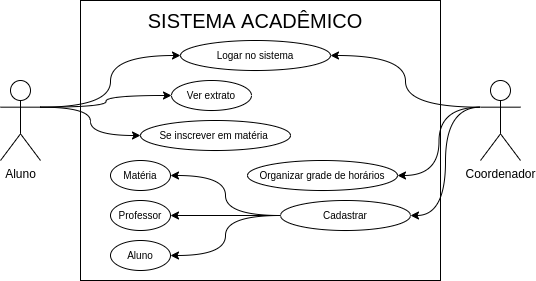
\includegraphics[scale=0.7]{Pictures/JV/Diagrama de caso de uso - aps.png}
                \label{casos_de_uso}
            \end{figure}    % IMAGEM CASOS DE USO
            
    \end{comment}
    \section{Modelagem do Sistema}
        Como forma de visualizar parte de como o sistema age internamente, algumas modelagens são feitas para que possam ser compreendidas visualmente, essas modelagens são de dois tipos: Processos e Dados.
        
        \subsection{Modelagem de Processos}
            Na modelagem de processos, vemos alguns dos processos que os usuários do sistema poderão utilizar.
            
            De uma forma geral, sempre teremos um usuário do sistema interagindo com o Sistema Acadêmico (Figura \ref{DFD1}).
            \begin{figure}[htbp]\centering
                \caption{Sistema Acadêmico simples}
                
\includegraphics[scale=0.7]{Pictures/JV/DFD/DFD - Sistema Acadêmico simples.png}
                \label{DFD1}
            \end{figure}    % IMAGEM DFD1
            
            O usuário para acessar o sistema, precisa utilizar seu e-mail e senha para fazer login. Tendo feito o login, ele pode requerer informações sobre as matérias (Figura \ref{DFD2}).
            \begin{figure}[htbp]\centering
                \caption{Sistema Acadêmico}
                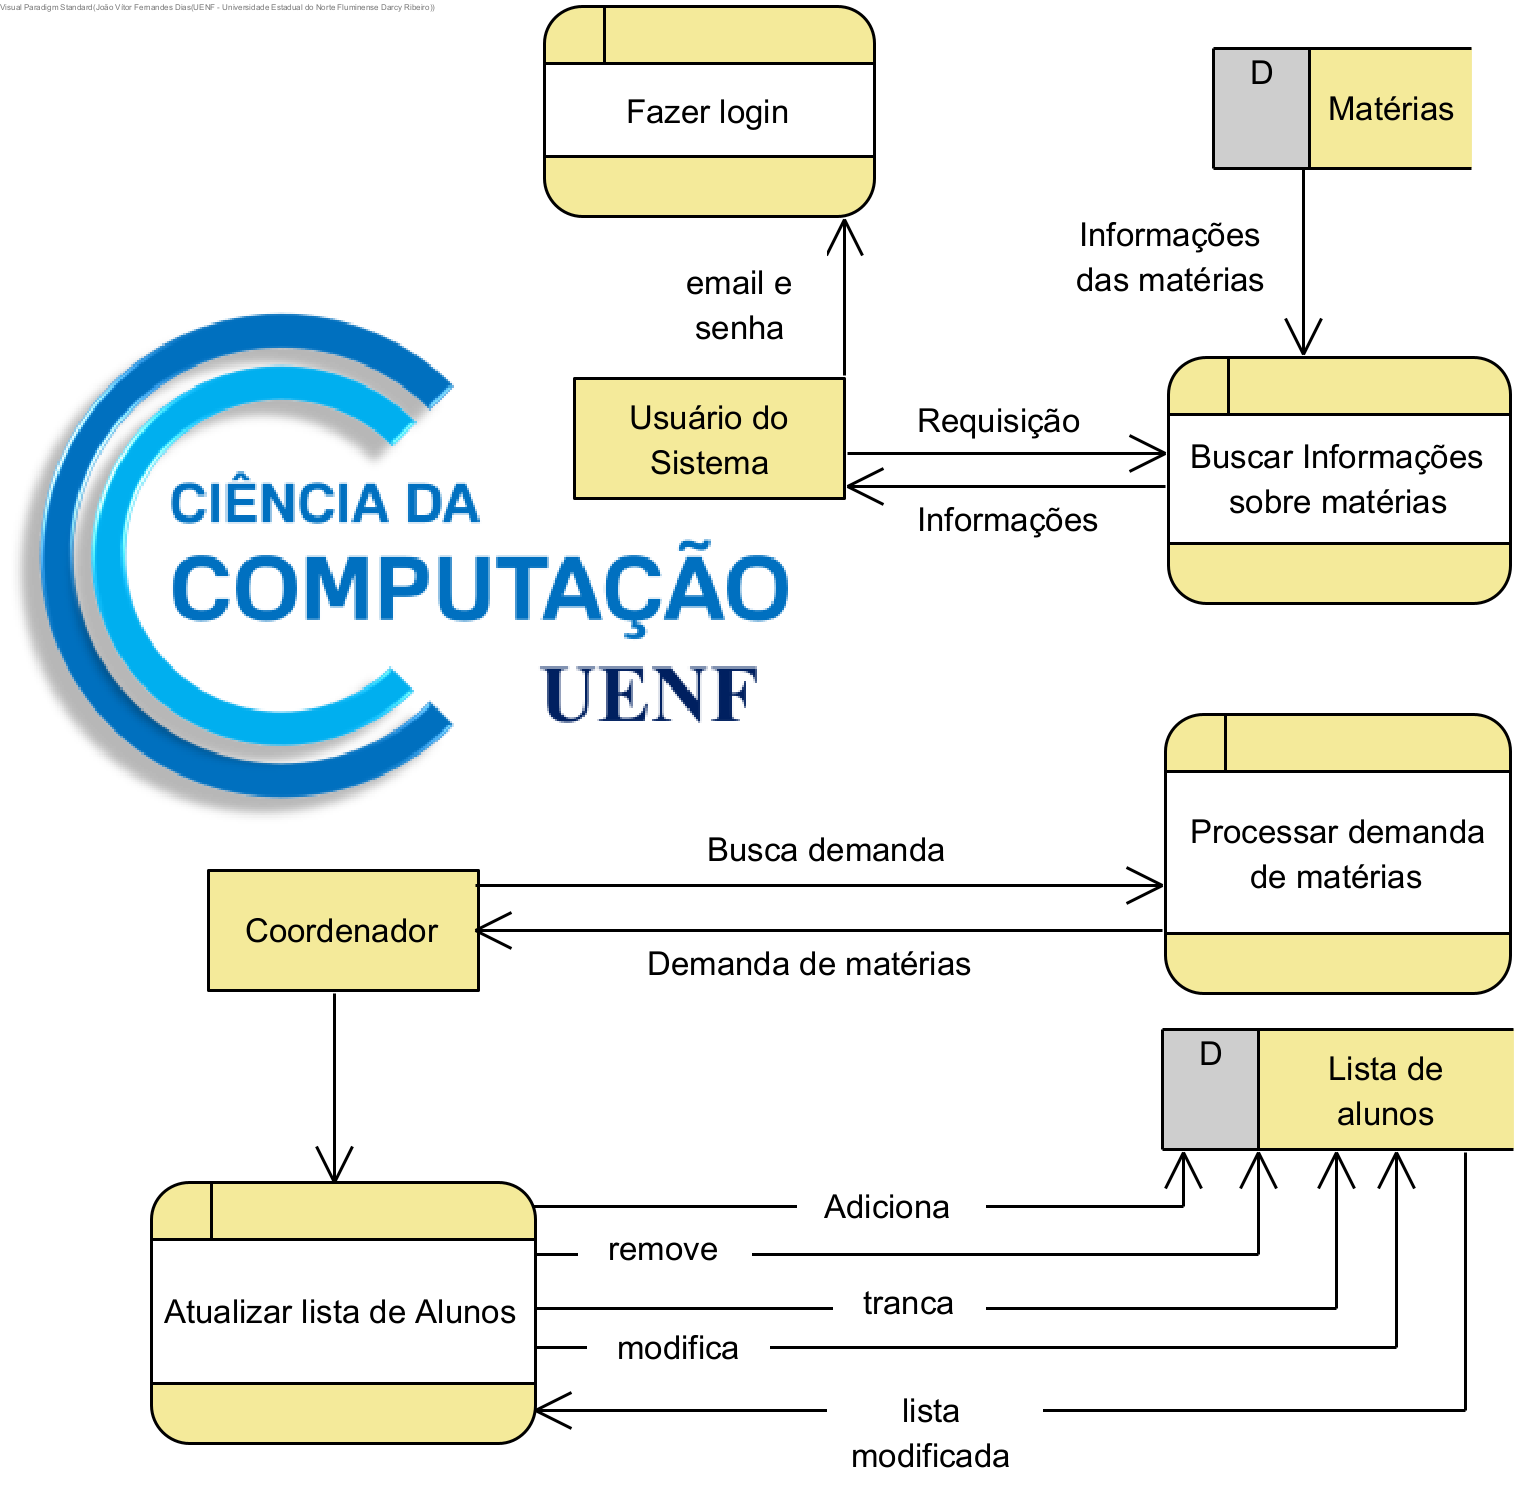
\includegraphics[scale=0.7]{Pictures/JV/DFD/DFD - Sistema Acadêmico.png}
                \label{DFD2}
            \end{figure}    % IMAGEM DFD2
            
            Já o coordenador consegue buscar quais são as matérias que os alunos demandam. Ele também tem a capacidade de atualizar a listagem de alunos. Ele pode adicionar, remover, trancar, modificar e obter a lista de alunos modificada (Figura \ref{DFD3}).
            \begin{figure}[htbp]\centering
                \caption{Processar demanda de matérias}
                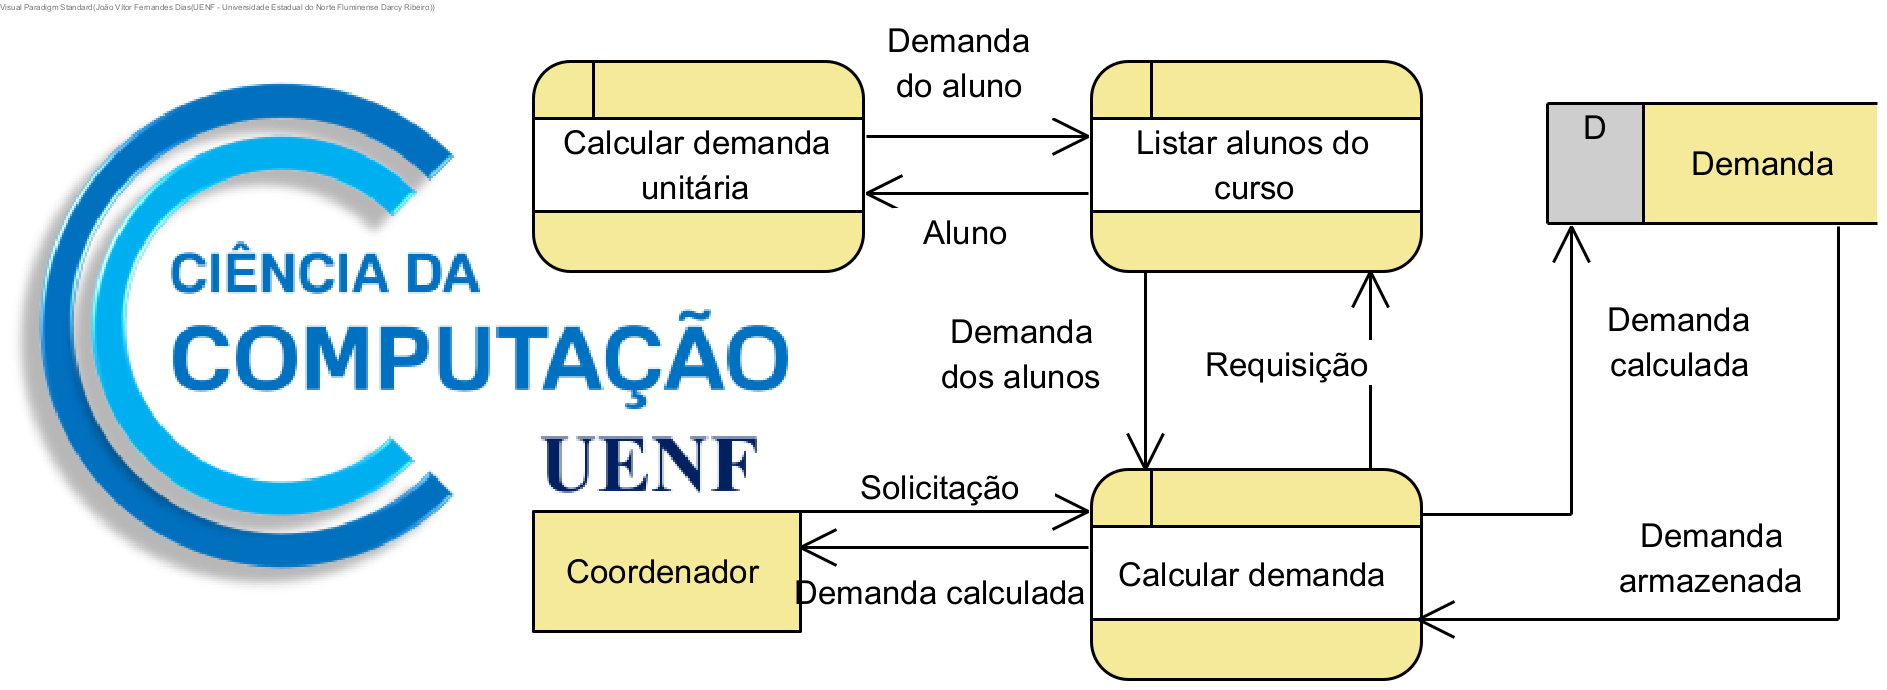
\includegraphics[scale=0.7]{Pictures/JV/DFD/DFD - Processar demanda de matérias.png}
                \label{DFD3}
            \end{figure}    % IMAGEM DFD3
        
        \subsection{Modelagem de Dados}
            Além de ter visualmente parte da forma como o sistema executa seus processos, podemos ver também a forma como o sistema armazenará os seus dados.
            
            Alguns dos dados presentes envolvendo as matérias são: o seu código, o código do professor que ministrará, a duração, o dia da semana, e o nome da matéria (Figura \ref{DFD1}).
            \begin{figure}[htbp]\centering
                \caption{Matéria disponível}
                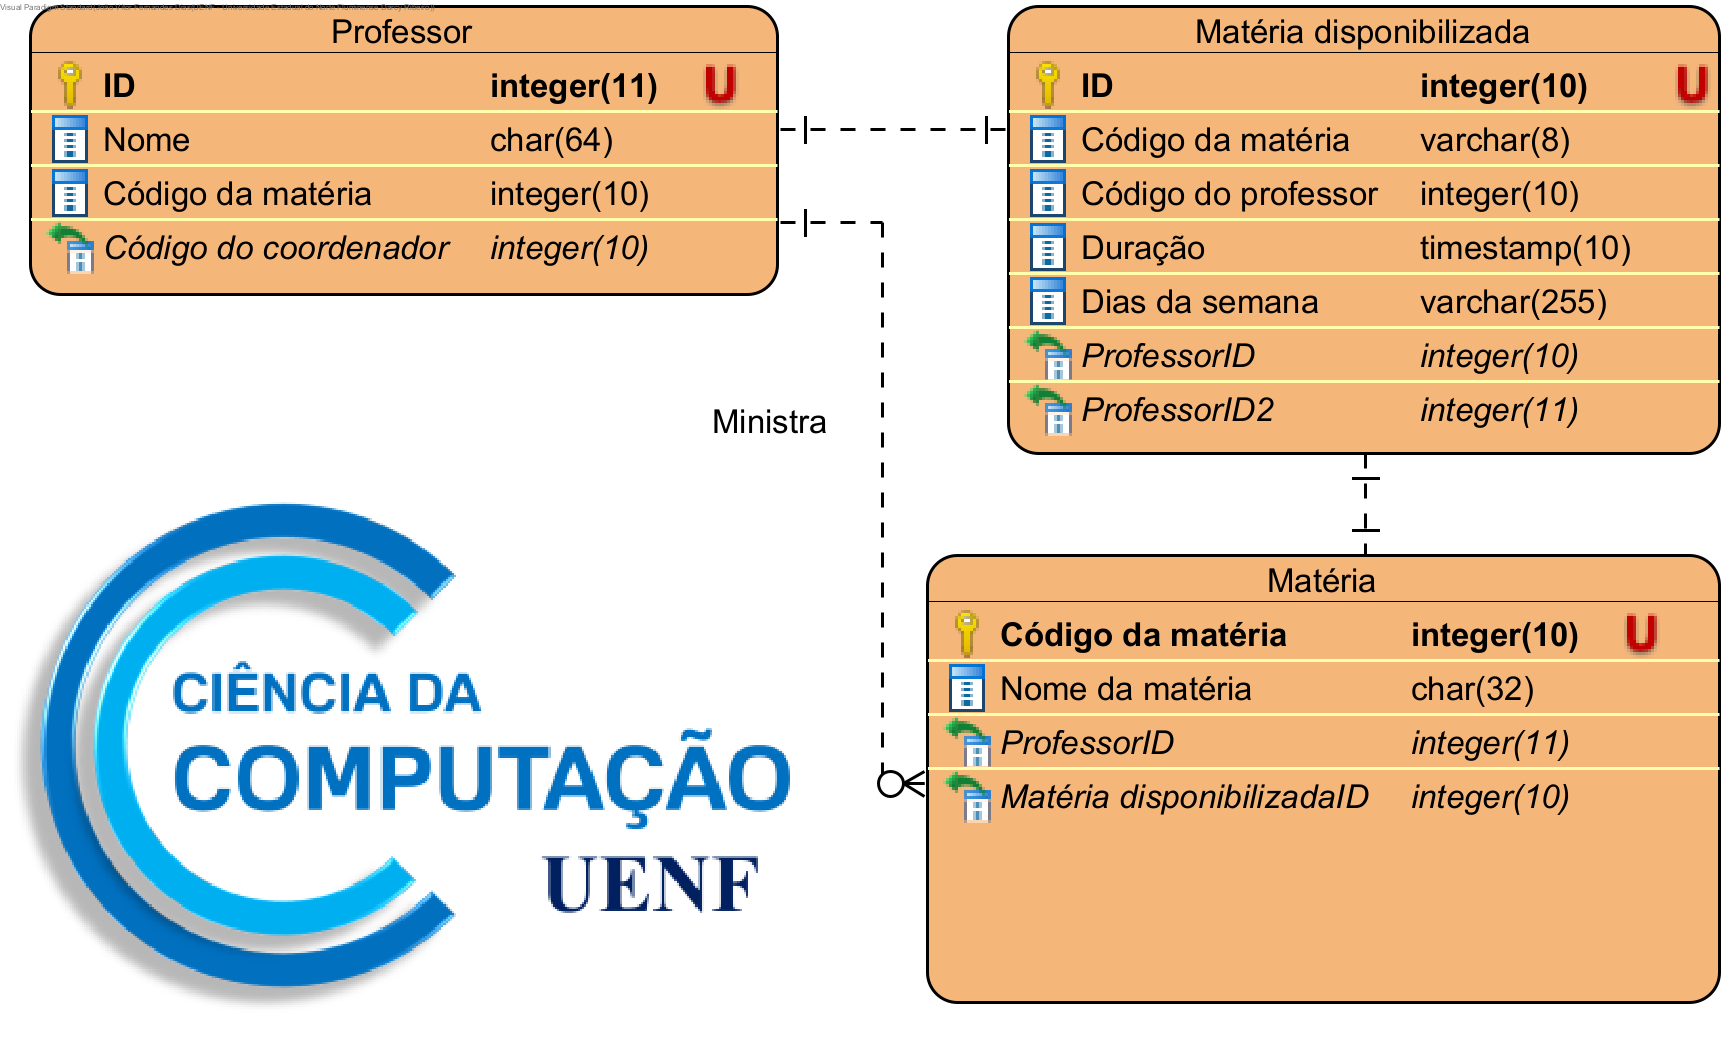
\includegraphics[scale=0.7]{Pictures/JV/DER/DER - Matéria disponivel.png}
                \label{DER1}
            \end{figure}    % IMAGEM DER1
            
            Os dados envolvendo as notas dos alunos têm relação com as provas que foram realizadas, em uma determinada hora, de um determinado bloco, em uma sala, para alunos de algum curso em algum semestre de algum ano (Figura \ref{DFD2}).
            \begin{figure}[htbp]\centering
                \caption{Notas}
                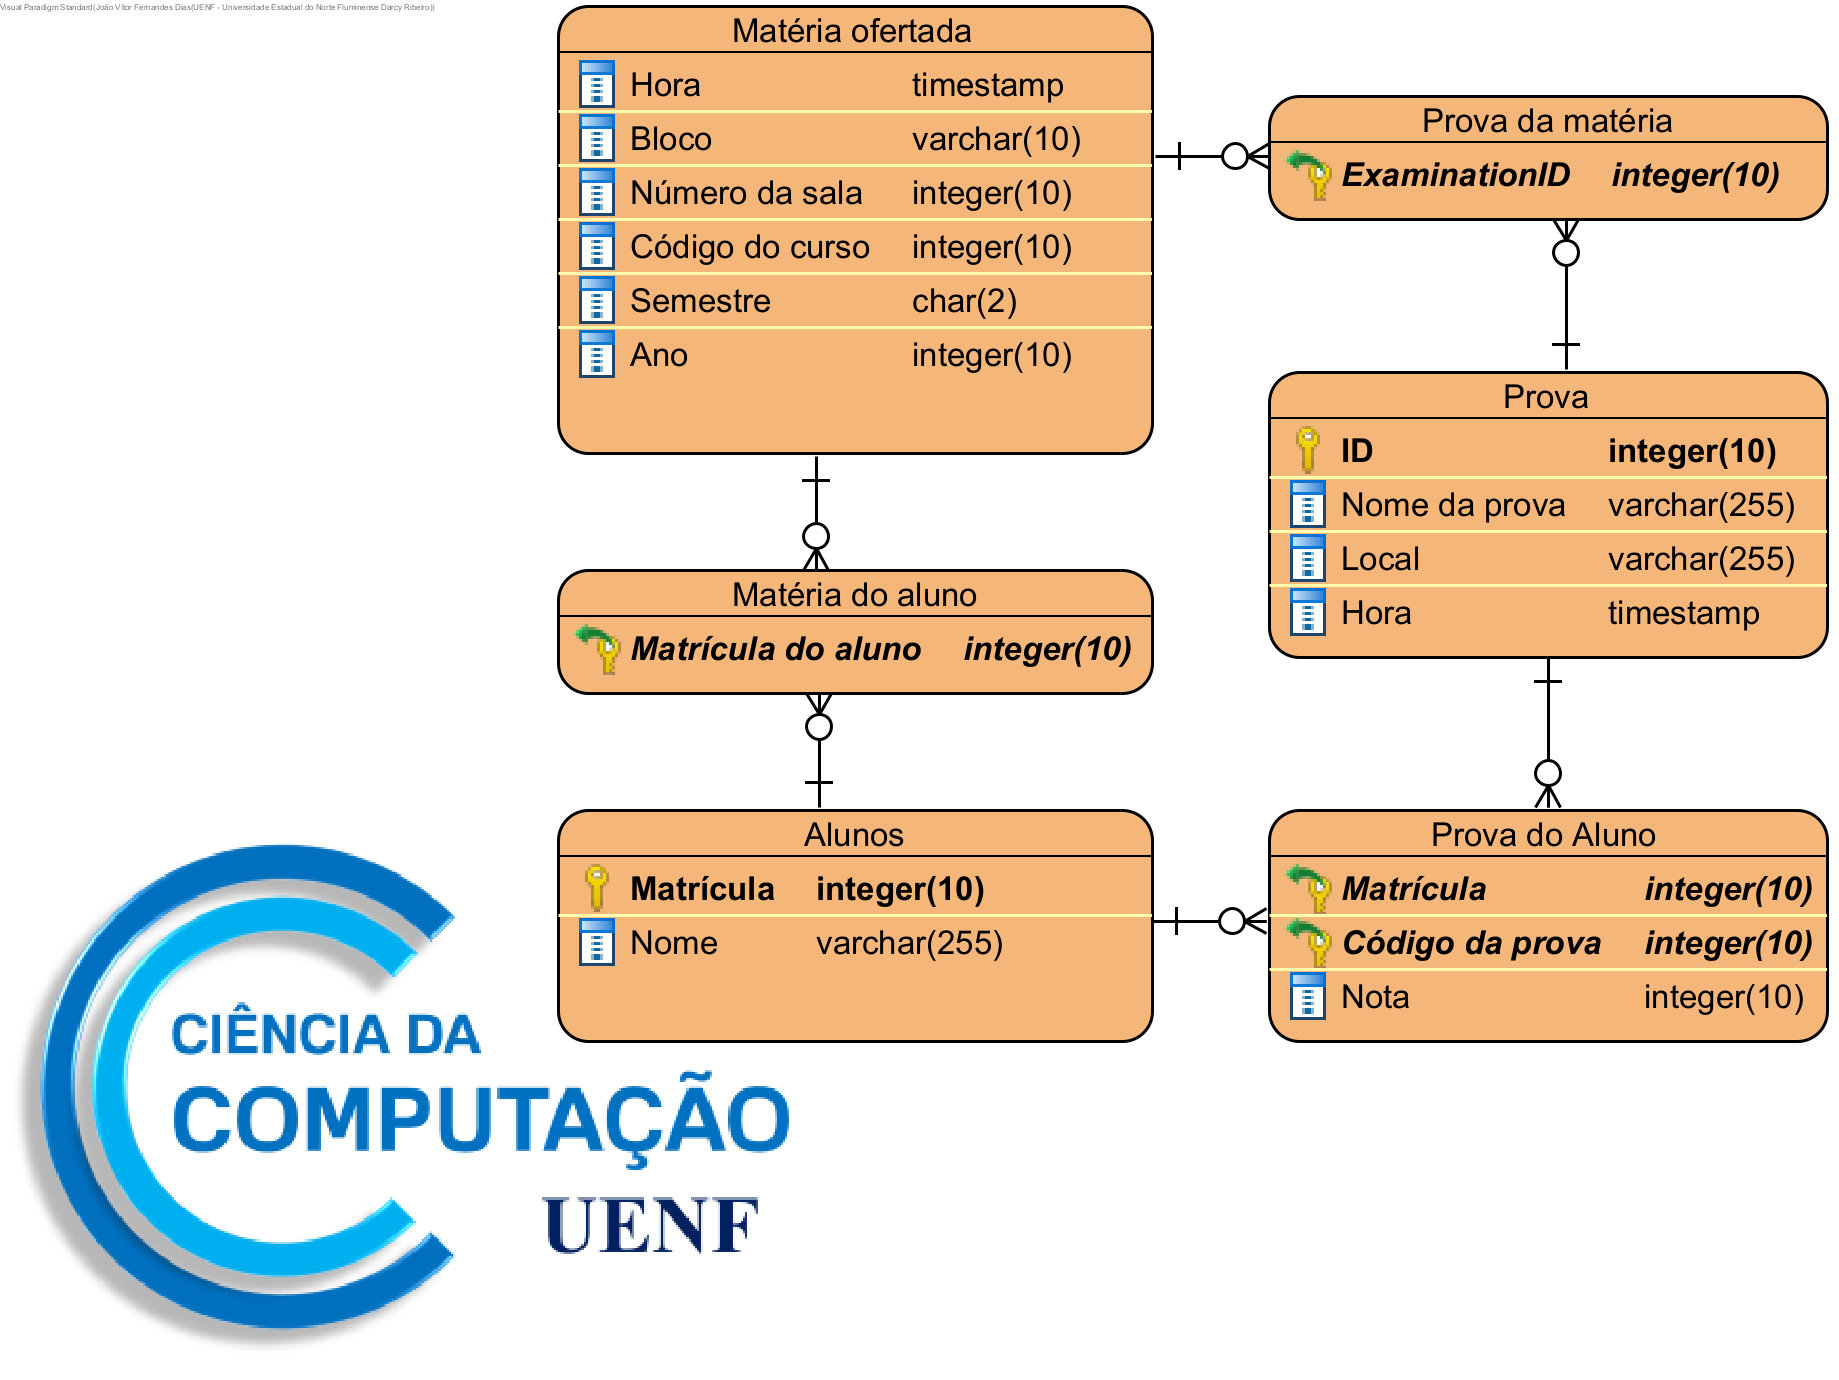
\includegraphics[scale=0.7]{Pictures/JV/DER/DER - Notas.png}
                \label{DER2}
            \end{figure}    % IMAGEM DER2
            
            Temos também as relações entre Alunos, professores e coordenadores. Os alunos têm nome e o código do curso, o aluno pode frequentar várias matérias que são ministradas por vários professores. Sendo cada matéria ministrada por somente um. O coordenador coordenada vários professores e vários alunos (Figura \ref{DFD3}).
            \begin{figure}[htbp]\centering
                \caption{Alunos, professores e coordenadores}
                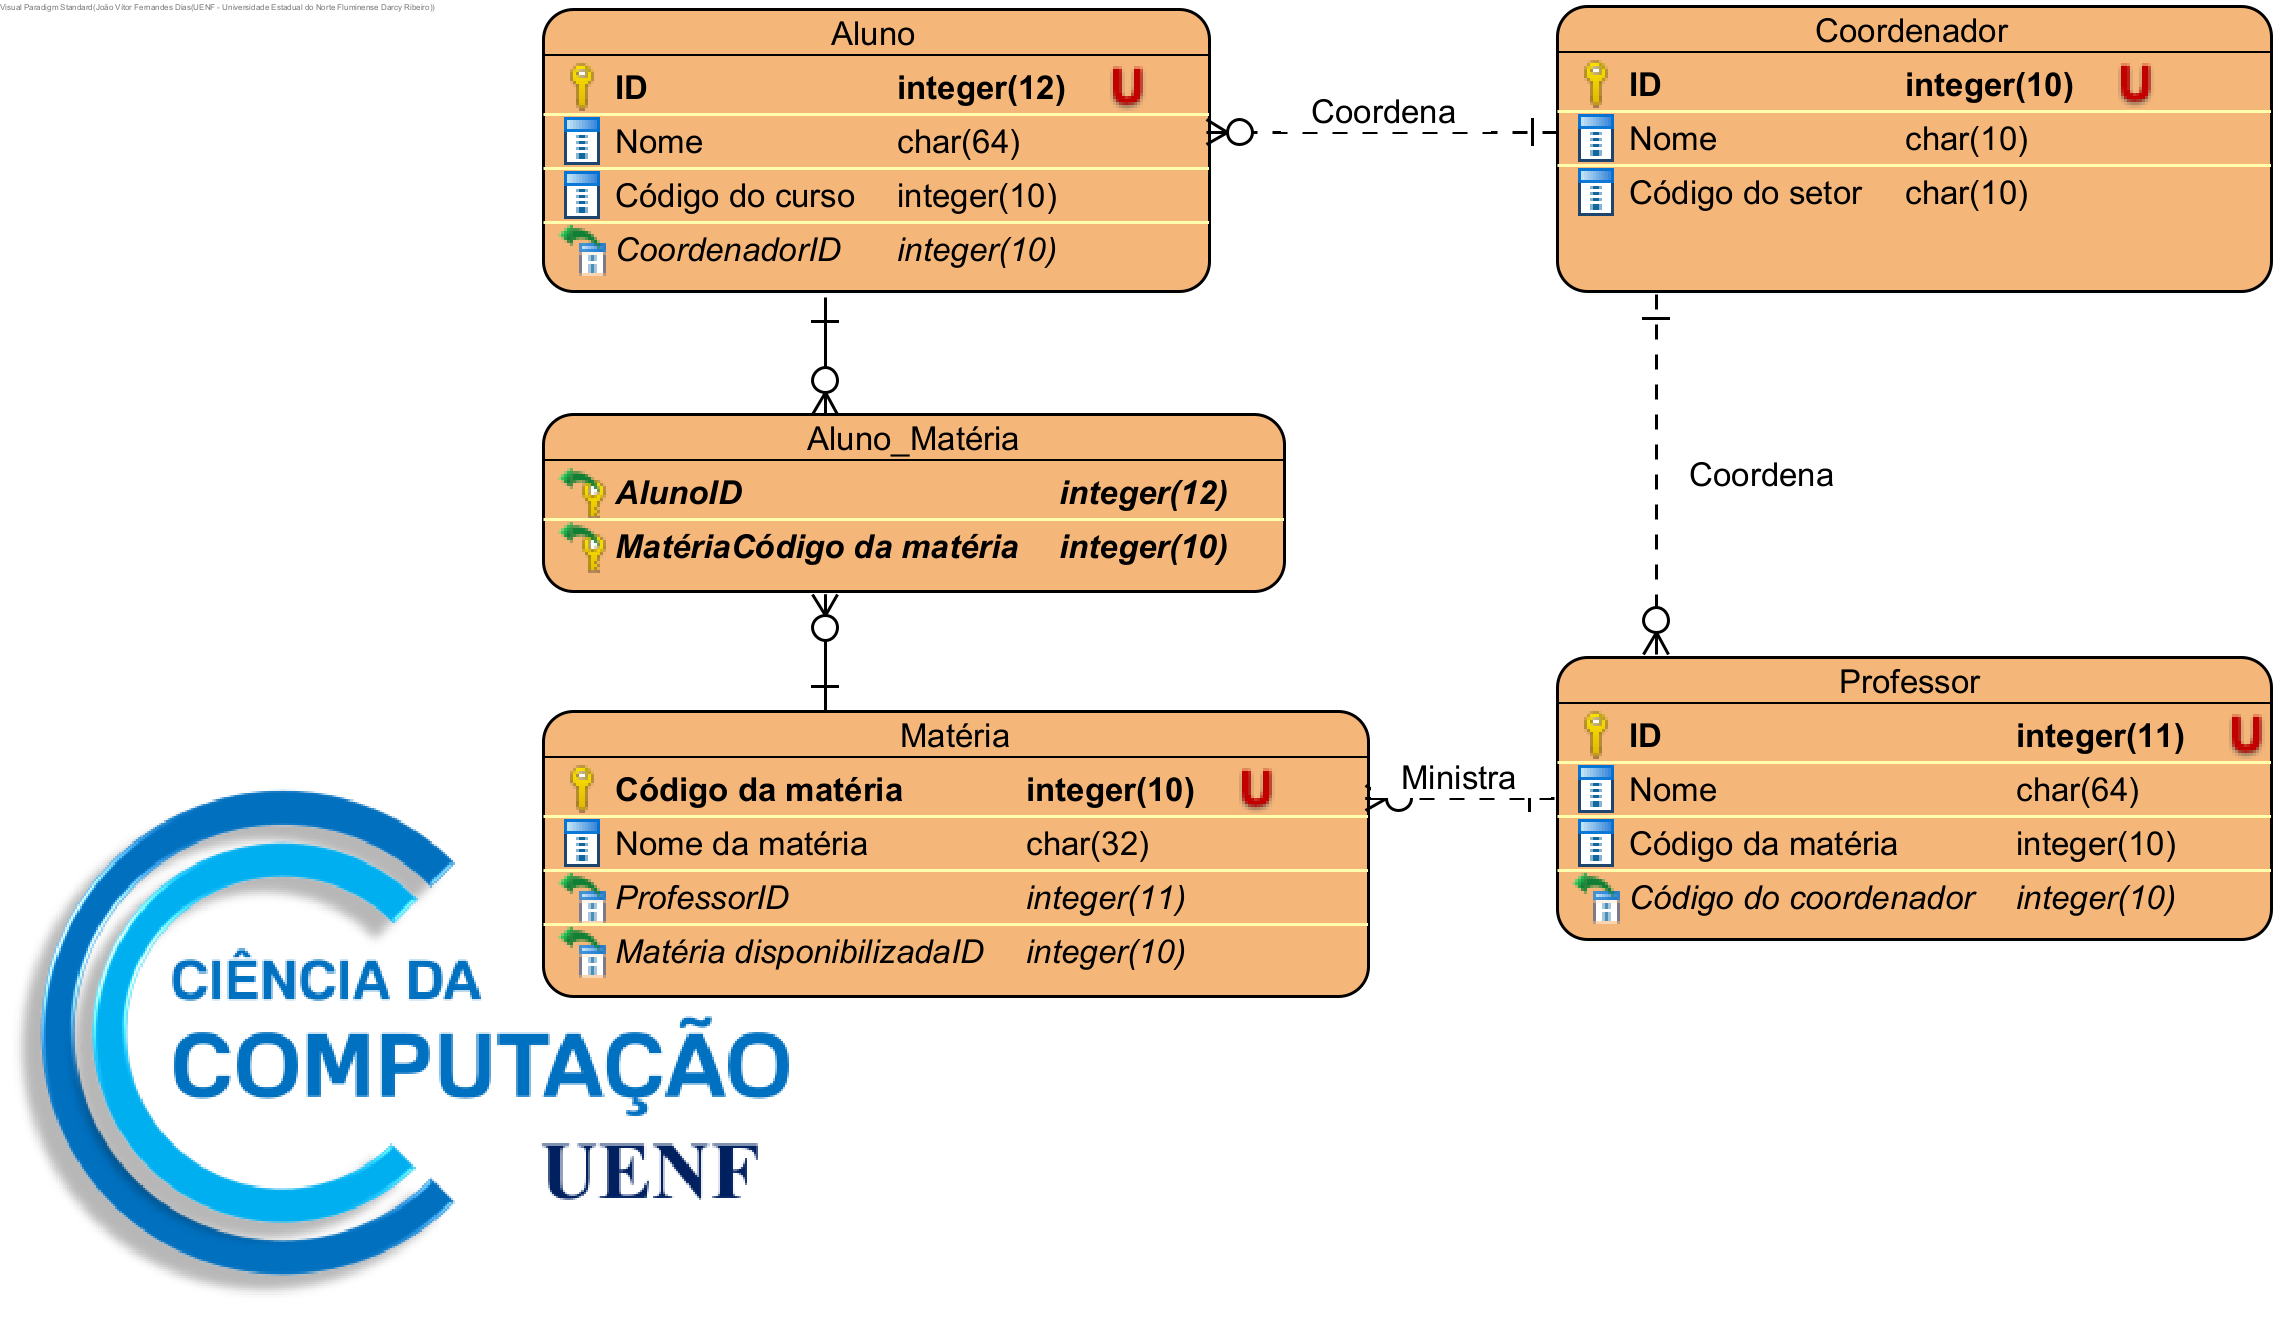
\includegraphics[scale=0.7]{Pictures/JV/DER/DER - Aluno_coord_prof.png}
                \label{DER3}
            \end{figure}    % IMAGEM DER3
